 \documentclass[10pt, table, dvipsnames,xcdraw, handout]{beamer}
\usetheme[progressbar=frametitle]{metropolis}
\usepackage{appendixnumberbeamer}
\usetikzlibrary{arrows.meta, positioning, quotes}
\usepackage[shortlabels]{enumitem}
\usepackage{xcolor}
\usepackage{mathtools}


\usepackage{cancel}

\newcommand\hcancel[2][black]{\setbox0=\hbox{$#2$}%
\rlap{\raisebox{.45\ht0}{\textcolor{#1}{\rule{\wd0}{1pt}}}}#2} 


\usepackage{booktabs}
\usepackage[scale=2]{ccicons}

\usepackage{pgfplots}
\usepgfplotslibrary{dateplot}

\usepackage{xspace}
\newcommand{\themename}{\textbf{\textsc{metropolis}}\xspace}
\newcommand{\cb}{\cellcolor{blue!25}}


% Notation:
\newcommand{\cT}{\ensuremath{\mathcal{T}}}
\newcommand{\cD}{\ensuremath{\mathcal{D}}}
\newcommand{\cX}{\ensuremath{\mathcal{X}}}
\newcommand{\cY}{\ensuremath{\mathcal{Y}}}
\newcommand{\cZ}{\ensuremath{\mathcal{Z}}}
\newcommand{\cH}{\ensuremath{\mathcal{H}}}
\newcommand{\cG}{\ensuremath{\mathcal{G}}}

\newcommand{\bR}{\ensuremath{\mathbb{R}}}
\newcommand{\bN}{\ensuremath{\mathbb{N}}}
\newcommand{\bP}{\ensuremath{\mathbb{P}}}
\newcommand{\bT}{\ensuremath{\mathbb{T}}}
\newcommand{\bL}{\ensuremath{\mathbb{L}}}

\newcommand{\bfX}{\ensuremath{\mathbf{X}}}
\newcommand{\bfY}{\ensuremath{\mathbf{Y}}}
\newcommand{\bfy}{\ensuremath{\mathbf{y}}}

% Tikz seys
\tikzset{cross/.style={cross out, draw, 
         minimum size=2*(#1-\pgflinewidth), 
         inner sep=0pt, outer sep=0pt}}

\title{Machine Learning I}
\subtitle{Lecture 5: Linear Methods in Classification}
% \date{\today}
\date{}
\author{Nathaniel Bade}
\institute{Northeastern University Department of Mathematics}
% \titlegraphic{\hfill\includegraphics[height=1.5cm]{logo.pdf}}

\begin{document}

\maketitle

\begin{frame}{Table of contents}
  \setbeamertemplate{section in toc}[sections numbered]
  \tableofcontents[hideallsubsections]
\end{frame}


%%%%%%%%%%%%%% Slidshow Start %%%%%%%%%%%%%% 


\section{Multilabel Classification}

\begin{frame}[fragile]{Multilable Classification: Notation}
  \begin{minipage}[t][0.5\textheight][t]{\textwidth}
	\centering \includegraphics[height=0.5\textheight]{L9Multilabel1.png} 
  \end{minipage}
  \vfill
\begin{minipage}[t][0.5\textheight][t]{\textwidth}
We will now expand our toolbox to include methods of classification for multiple labels. \pause Suppose there are $|\cG| = K$ classes, labeled $1,2,\ldots, K$. Let $Y_k$ be the \textbf{indicator} function for $k$, that is $Y_k = 1$ if $G= k$, but is 0 otherwise. \pause

These variables are collected together into a vector  $Y = (Y_1,\ldots, Y_K)\in \mathbb{R}^K$. The $N$ training instances then form an $N\times K$ matrix $\mathbf{Y}$.  
\end{minipage}
\end{frame}


\begin{frame}[fragile]{Multilable Classification: Notation}
  \begin{minipage}[t][0.5\textheight][t]{\textwidth}
	\centering \includegraphics[height=0.5\textheight]{L9Multilabel1.png} 
  \end{minipage}
  \vfill
\begin{minipage}[t][0.5\textheight][t]{\textwidth}
A model $Y = \hat{f}(X)$ will give a probability for each $Y_k$ for each point $X$ in the domain. Letting
$$
\hat{f}(X) = (\hat f_1(X),\ldots, \hat f_K(X))\,\hspace{1em}\text{given}\hspace{1em} \hat f_1(X)+\ldots+ \hat f_K(X) = 1\,,\, \hat f_k(X)\geq0\,,
$$
we have $\hat{f}(X)\in \mathbb{R}^K$, with $\hat{f}_k(X) = \hat{Y}_k = \mathbb{P}(Y = k| X = X)$ be the probability that $Y$ takes the label $k$ given $X$.
\end{minipage}
\end{frame}







\begin{frame}[fragile]{Multilabel Classification}
  \begin{minipage}[t][0.5\textheight][t]{\textwidth}
	\centering \includegraphics[height=0.5\textheight]{L9Multilabel2.png} 
  \end{minipage}
  \vfill
\begin{minipage}[t][0.5\textheight][t]{\textwidth}
For each datapoint $(x_i, y_i)$, this means that $y_i = k$ is now encoded in a $K$ vector, where the $k$'th entry is 1 and the other entries are 0. If we encode this bitwise it is known as a \textbf{one-hot encoding}. \pause If probability functions $\hat f_k$ have been fit, a label $\hat y_i$ can be predicted by taking
$$
\hat G(x_i) = \underset{k\in \cG}{\text{argmax }} \hat f_k(x_i)
$$
\end{minipage}
\end{frame}





\begin{frame}[fragile]{Multilabel Classification}
  \begin{minipage}[t][0.5\textheight][t]{\textwidth}
	\centering \includegraphics[height=0.5\textheight]{L9BC1.png} 
  \end{minipage}
  \vfill
\begin{minipage}[t][0.5\textheight][t]{\textwidth}
As a first example, in the plot above we are trying to separate cells into malignant and benign by their mean area and concavity. We have two labels, so $Y\in \mathbb{R}^2$, with $Y_1$ the probability that a cell with features $X$ is malignant and $Y_2$ the probability it is benign. 

\end{minipage}
\end{frame}


\begin{frame}[fragile]{Multilabel Classification}
  \begin{minipage}[t][0.5\textheight][t]{\textwidth}
	\centering \includegraphics[height=0.5\textheight]{L9BC3.png} 
  \end{minipage}
  \vfill
\begin{minipage}[t][0.5\textheight][t]{\textwidth}
Fitting an affine linear function to $Y$ takes the same form as before:
$$
Y = [Y_1,\ldots, Y_k] = X^T\beta\,,
$$
only now $\beta \in \mathbf{p+1\times K}$ is a $p+1\times K$ matrix. Minimize $RSS$ for each of the columns of $\mathbf{Y}$ yields $\beta = (\mathbf{X}^T\mathbf{X})^{-1}\mathbf{X}^T\mathbf{Y}$, provided we bound $Y_k\in [0,1]$. 
\end{minipage}
\end{frame}



\begin{frame}[fragile]{Multilabel Classification}
  \begin{minipage}[t][0.5\textheight][t]{\textwidth}
	\centering \includegraphics[height=0.5\textheight]{L9BC3.png} 
  \end{minipage}
  \vfill
\begin{minipage}[t][0.5\textheight][t]{\textwidth}
In the cancer classification above, we see a hard line called the \textbf{decision boundary}. This is the line where $\hat{Y}_1 = \hat{Y}_2 = .5$, and it separates the portion of the domain for $X$ most probably takes on label $k$ and label $j$. 
\end{minipage}
\end{frame}


\begin{frame}[fragile]{Multilabel Classification}
  \begin{minipage}[t][0.5\textheight][t]{\textwidth}
	\centering \includegraphics[height=0.5\textheight]{L9BC3.png} 
  \end{minipage}
  \vfill
\begin{minipage}[t][0.5\textheight][t]{\textwidth}
Note: The most natural loss function for a categorical variable is simple the 0-1 loss function, that is 1 if $y_i = \text{argmax}_k(\hat{f}_k(x_i))$ and 0 otherwise. 

However, 0-1 loss is discrete, and as a result is very difficult to optimize using smooth methods. Working instead with the probabilities makes optimization more straightforward. 
\end{minipage}
\end{frame}





\section{Regression on Categorical Variables}


\begin{frame}[fragile]{Multilable Regression}
Given a classification problem with $K$ labels, we encode the repose categories $\mathcal{G}$ into a $K$ vector $Y = (Y_1,\ldots, Y_K)$, $Y_i\in \{0,1\}$. The $N$ training instances form a $N\times K$ matrix $\bfY$ of 1's and 0's. \pause Letting $X$ denote the $p+1$ vector with $X_0 = 1$ as usual, the linear model
$$
Y = X^T\beta\,,
$$\pause
now has a $p+1\times K$ matrix of coefficients $\beta$. The loss for each column is a $K$ vector
$$
RSS(\beta) = \sum_{i=1}^N (y_i-\hat{f}(x_i))^T(y_i-\hat{f}(x_i)) = (\mathbf{Y} - \mathbf{X}\beta)^T(\mathbf{Y} - \mathbf{X}\beta)\,,
$$
minimizing all columns simultaneously gives $\hat \beta = (\bfX^T\bfX)^{-1}\bfX^T\bfY$.

\end{frame}



\begin{frame}[fragile]{Multilable Regression}
With a little bit of work (\textbf{exercise}, use centered vectors) one can show that 
$$
\sum_{k=1}^K \hat f_k(X) = 1\hspace{1em}\forall X\,,
$$
but there is no guarantee that the $\hat f_k$ are positive. \pause This isn't necessarily fatal, in fact this kind of linear regression often works well, but we shouldn't understand the $\hat f_k$ as providing strict probabilities in any sense. 
\end{frame}



\begin{frame}[fragile]{Multilabel Classification: Example}
  \begin{minipage}[t][0.5\textheight][t]{\textwidth}
	\centering \includegraphics[height=0.5\textheight]{L9Multilabel4.png} 
  \end{minipage}
  \vfill
\begin{minipage}[t][0.5\textheight][t]{\textwidth}
Also, while a linear decision boundary may not provide the best fit they have low variance relative to other classes. \pause The regions above are defined by the regions in which $\hat f_k(x)$ is the largest for each $k$. The lines are the intersection lines $\hat f_k=\hat f_j$. 
\end{minipage}
\end{frame}



\begin{frame}[fragile]{Multilabel Classification: Example}
  \begin{minipage}[t][0.5\textheight][t]{\textwidth}
	\centering \includegraphics[height=0.5\textheight]{L9Multilabel5.png} 
  \end{minipage}
  \vfill
\begin{minipage}[t][0.5\textheight][t]{\textwidth}
Also, while a linear decision boundary may not provide the best fit they have low variance relative to other classes. The regions above are defined by the regions in which $\hat f_k(x)$ is the largest for each $k$. The lines are the intersection lines $\hat f_k=\hat f_j$. 
\end{minipage}
\end{frame}



\begin{frame}[fragile]{Multilabel Classification: Example}
  \begin{minipage}[t][0.5\textheight][t]{\textwidth}
	\centering \includegraphics[height=0.5\textheight]{L9Multilabel6.png} 
  \end{minipage}
  \vfill
\begin{minipage}[t][0.5\textheight][t]{\textwidth}
Also, while a linear decision boundary may not provide the best fit they have low variance relative to other classes. The regions above are defined by the regions in which $\hat f_k(x)$ is the largest for each $k$. The lines are the intersection lines $\hat f_k=\hat f_j$. 
\end{minipage}
\end{frame}




\begin{frame}[fragile]{Multilabel Classification: Masking}
  \begin{minipage}[t][0.5\textheight][t]{\textwidth}
	\centering \includegraphics[height=0.5\textheight]{L9LinAnal.png} 
  \end{minipage}
  \vfill
\begin{minipage}[t][0.5\textheight][t]{\textwidth}
The biggest problem with linear decision boundaries comes from masking. In the admittedly extreme example on the left, the three clusters are clearly distinct but the linear regressor misses the middle class completely. \pause On the right we see the classes being successfully fit with a quadratic regression. 
\end{minipage}
\end{frame}


\begin{frame}[fragile]{Multilabel Classification: Quadratic Fitting}
A quick note about quadratic regression. While we will say more about nonlinear fitting later, quadratic regression can be though of a linear regression on the constructed features $X_iX_j$, for all $i,j$. If we're willing to add $p(p+1)/2$ new variables the quadratic regression
$$
Y = \beta_0 + \sum_{i}X_i\beta_i + \sum_{i<j}X_iX_j\alpha_{ij}
$$
can be done with a linear fit. 
\end{frame}


\section{Linear Discriminant Analysis}



\begin{frame}[fragile]{Class Conditional Density}
  \begin{minipage}[t][0.5\textheight][t]{\textwidth}
	\centering \includegraphics[height=0.5\textheight]{L5MultNorm.png} 
  \end{minipage}
  \vfill
\begin{minipage}[t][0.5\textheight][t]{\textwidth}
Consider a mixture model like the one show above, where each of the labels is distributed as a multivariate normal distribution. The \textbf{class conditional density} 
$$
f_k(x) = \bP(X=x|G=k)\,,
$$
is the multivariate normal distribution for the $k$'th label.
\end{minipage}
\end{frame}


\begin{frame}[fragile]{Class Conditional Density}
  \begin{minipage}[t][0.5\textheight][t]{\textwidth}
	\centering \includegraphics[height=0.5\textheight]{L1PairOfGuassians.png} 
  \end{minipage}
  \vfill
\begin{minipage}[t][0.5\textheight][t]{\textwidth}
Consider a mixture model like the one show above, where each of the labels is distributed as a multivariate normal distribution. The \textbf{class conditional density} 
$$
f_k(x) = \bP(X=x|G=k)\,,
$$
is the multivariate normal distribution for the $k$'th label. Above are the normal $f_k$ viewed as functions. 
\end{minipage}
\end{frame}



\begin{frame}[fragile]{Bayes Theorem and Class Densities}
We  are interested in estimating the conditional probabilities $P(G = k|X = x)$. Out first step of course should be to total the number of labels for each class in our training set, giving us a (\textbf{prior}) probability $\pi_k$ for each label. \pause Since the class conditional density
$$
f_k(x) = \bP(X=x|G=k)\,,
$$
is the distribution of $x$'s for the label $k$, Bayes theorem gives the probability for a label $k$ at a point $x$:
$$
\bP(G=k|X=x) = \frac{\bP(G=k) \bP(X=x|G=k)}{\bP(X=x)} = \frac{ \pi_k \, f_k(x)}{\sum_{j=1}^K\,\pi_j}\, f_j(x)\,.
$$\pause
So knowing $f_k(x)$ and estimating the label proportions is almost good enough to know $\bP(G|X)$. 
\end{frame}







\begin{frame}[fragile]{Bayes Theorem and Class Densities}
Many techniques are based on models for the class densities:
\begin{itemize}
\item[] If we assume the class density function are Gaussian, this leads to linear and quadratic class boundaries. This process is known as Linear or Quadratic discriminant analysis in reference to the class boundary shape. \pause
\item[] We will also see that we can generate linear class boundaries without the Gaussian assumption by fitting linear functions to the probabilities directly, while forcing the result to be a real probability vector. This is known as logistic regression. 
\pause
\item[] Finally, we can generate class densities with nonlinear boundaries by using non-parametric density estimates (ie sampled or bootstrapped densities).\pause
\end{itemize}

We will show the first point now, that if the class conditional densities are Gaussian, the decision boundaries must be linear or quadratic.
\end{frame}




\begin{frame}[fragile]{Gaussian Densities}
  \begin{minipage}[t][0.5\textheight][t]{\textwidth}
	\centering \includegraphics[height=0.5\textheight]{L9Multilabel1.png} 
  \end{minipage}
  \vfill
\begin{minipage}[t][0.5\textheight][t]{\textwidth}
Given a multilabel classification problem, we may try to model each of the labels directly by guess their underlying probability distribution and using maximum likelihood, or other methods. 
\end{minipage}
\end{frame}





\begin{frame}[fragile]{Gaussian Densities}
  \begin{minipage}[t][0.5\textheight][t]{\textwidth}
	\centering \includegraphics[height=0.5\textheight]{L9MultivariateNormal.png} 
  \end{minipage}
  \vfill
\begin{minipage}[t][0.5\textheight][t]{\textwidth}
Suppose we model each density $f_k(x)$ as a multivariate Gaussian with covariance matrix $\mathbf{\Sigma}_k$
$$
f_k(x) = \big[(2\pi)^p |\mathbf{\Sigma}_k| \big]^{-\frac12}\exp\left(\,-\frac12(x-\mu_k)^T\mathbf{\Sigma}_k^{-1}(x-\mu_k)  \,\right)\,.
$$
\end{minipage}
\end{frame}



\begin{frame}[fragile]{Gaussian Densities}
  \begin{minipage}[t][0.5\textheight][t]{\textwidth}
	\centering \includegraphics[height=0.5\textheight]{L9MultivariateNormal.png} 
  \end{minipage}
  \vfill
\begin{minipage}[t][0.5\textheight][t]{\textwidth}
$$
f_k(x) = \big[(2\pi)^p |\mathbf{\Sigma}_k| \big]^{-\frac12}\exp\left(\,-\frac12(x-\mu_k)^T\mathbf{\Sigma}_k^{-1}(x-\mu_k)  \,\right)
$$
Above are the $3\sigma$ ellipse and marginal distributions for
$$
\mu_k= 
\left(
\begin{matrix}
0\\0
\end{matrix}
\right)
\hspace{1em}
\mathbf{\Sigma} = 
\left(
\begin{matrix}
1&3/5\\
3/5&2
\end{matrix}
\right)\,.
$$
\end{minipage}
\end{frame}





\begin{frame}[fragile]{Gaussian Densities}
  \begin{minipage}[t][0.5\textheight][t]{\textwidth}
	\centering \includegraphics[height=0.5\textheight]{L9MultivariateNormal2.png} 
  \end{minipage}
  \vfill
\begin{minipage}[t][0.5\textheight][t]{\textwidth}
The eigenvectors $e_i$ of $\mathbf{\Sigma}$ define the axes off the ellipsoid, the axis length is $\sqrt{\lambda_i}$. This is a direct result of the eigen-decomposition
$$
\mathbf{\Sigma} = UDU^T
$$
which always exists because $\mathbf{\Sigma}$ is real and symmetric.
\end{minipage}
\end{frame}





\begin{frame}[fragile]{Gaussian Densities}
Suppose we model each density $f_k(x)$ as a multivariate Gaussian with covariance matrix $\mathbf{\Sigma}_k$
$$
f_k(x) = \big[(2\pi)^p |\mathbf{\Sigma}_k| \big]^{-\frac12}\exp\left(\,-\frac12(x-\mu_k)^T\mathbf{\Sigma}_k^{-1}(x-\mu_k)  \,\right)\,.
$$\pause\newline

We would like to characterize when $\mathbb{P}(G = k|X = x)$ is greater than $\mathbb{P}(G = j|X = x)$, for each $k$ and $j$. Given the exponential, it's natural to compare the ratio of the logs. Using Bayes Theomre,  $k$ is more likely when 
$$
\log \frac{\bP(G=k|X=x)}{\bP(G= j|X=x)} = \log \frac{\pi_k f_k}{\pi_j f_j} > 0\,.
$$
\end{frame}




\begin{frame}[fragile]{Linear Discriminant Functions}
If the covaraince matrices are the same for each $k$, that is $\mathbf{\Sigma}_k = \mathbf{\Sigma}$ for all $k$, then 
$$
f_k(x) = \big[(2\pi)^p |\mathbf{\Sigma}| \big]^{-\frac12}\exp\left(\,-\frac12(x-\mu_k)^T\mathbf{\Sigma}^{-1}(x-\mu_k)  \,\right)\,.
$$\pause
and both the constant and quadratic terms cancel
\begin{align*}
\log\frac{f_k\pi_k}{f_j\pi_j} & = \log \frac{\pi_k}{\pi_j} - \frac12(x-\mu_k)^T\mathbf{\Sigma}^{-1}(x-\mu_k) + \frac12(x-\mu_j)^T\mathbf{\Sigma}^{-1}(x-\mu_j)
\\
\action<+->{&=  \log \frac{\pi_k}{\pi_j} - \frac12(\mu_k+\mu_j)^T\mathbf{\Sigma}^{-1}(\mu_k-\mu_j)  + x^T\mathbf{\Sigma}^{-1}(\mu_k-\mu_j) }
\\
\action<+->{&\geq  0\,.}
\end{align*}
\action<+->{This is a linear expression in $x$ and so leads to linear decision boundaries.}
\end{frame}



\begin{frame}[fragile]{Linear Discriminant Functions}
The equation
$$
0 \geq  \log \frac{\pi_k}{\pi_j} - \frac12(\mu_k+\mu_j)^T\mathbf{\Sigma}^{-1}(\mu_k-\mu_j)  + x^T\mathbf{\Sigma}^{-1}(\mu_k-\mu_j) 
$$\pause
can be rewritten as 
$$
\delta_k(x) \geq \delta_k(x)\,,
$$\pause
where
$$
\delta_k(x) = 
\log (\pi_k) - \frac12\mu_k^T\mathbf{\Sigma}^{-1}\mu_k  + x^T\mathbf{\Sigma}^{-1}\mu_k \,.
$$\pause

The label on $x$ is given by $\text{argmax}_k \delta_k(x)$. The linear decision boundaries are $\delta_k(x) = \delta_j(x)$. 
\end{frame}




\begin{frame}[fragile]{Linear Discriminant Functions}
  \begin{minipage}[t][0.5\textheight][t]{\textwidth}
	\centering \includegraphics[height=0.5\textheight]{L9LinearDecBoundry.png} 
  \end{minipage}
  \vfill
\begin{minipage}[t][0.5\textheight][t]{\textwidth}
The label on $x$ is given by $\text{argmax}_k \delta_k(x)$. The linear decision boundaries are $\delta_k(x) = \delta_j(x)$. \pause Above, we see three Gaussian distributions 95\% density contours, as well as the decision boundaries. 
\end{minipage}
\end{frame}




\begin{frame}[fragile]{Linear Discriminant Functions}
  \begin{minipage}[t][0.5\textheight][t]{\textwidth}
	\centering \includegraphics[height=0.5\textheight]{L9LinearDecBoundry.png} 
  \end{minipage}
  \vfill
\begin{minipage}[t][0.5\textheight][t]{\textwidth}
In practice, we need to estimate the parameters of the Gaussian distribution as follows: For each label $k$,
\begin{itemize}
\item[] $\hat{\pi}_k = N_k/N$, where $N_k$ is the number of observations of $k$. \pause
\item[] $\hat\mu_k  = \frac{1}{N_k}\sum_{y_i = k} x_i$ is the mean of $k$ observations.\pause
\item[] $\hat{\mathbf{\Sigma}}_k = \textbf{Var}(x_i)$ for $y_i = k$, is the sample covariance matrix.
\end{itemize}
\end{minipage}
\end{frame}







\begin{frame}[fragile]{Linear Discriminant Functions}
  \begin{minipage}[t][0.5\textheight][t]{\textwidth}
	\centering \includegraphics[height=0.5\textheight]{L9LinearDecBoundry.png} 
  \end{minipage}
  \vfill
\begin{minipage}[t][0.5\textheight][t]{\textwidth}
For binary classification it can be shown that the coefficient vector $\beta$ from least squares is proportional to the coefficient vector of linear discriminant analysis (LDA). But the origin $\beta_0$ might be different. \pause

For more labels, the correspondence between LDA and regression can be made by changing the loss function. This again shows the versatility of regression, since LDA can be shown to avoid masking problems. 
\end{minipage}
\end{frame}





\begin{frame}[fragile]{Quadratic Discriminant Functions}
  \begin{minipage}[t][0.5\textheight][t]{\textwidth}
	\centering \includegraphics[height=0.5\textheight]{L9QuadDecBoundry.png} 
  \end{minipage}
  \vfill
\begin{minipage}[t][0.5\textheight][t]{\textwidth}
If we remove the requirement that the $\mathbf{\Sigma}_k$ are all equal, the discriminant functions become quadratic
$$
\delta_k(x) = -\frac12\log|\mathbf{\Sigma}_k| - \frac12 (x-\mu_k)^T\mathbf{\Sigma}_k^{-1}(x-\mu_k) + \log \pi_k\,.
$$\pause
This is known as \textbf{quadratic discriminant analysis} (QDA).
\end{minipage}
\end{frame}






\begin{frame}[fragile]{Quadratic Discriminant Functions}
  \begin{minipage}[t][0.5\textheight][t]{\textwidth}
	\centering \includegraphics[height=0.5\textheight]{L9QuadDecBoundry.png} 
  \end{minipage}
  \vfill
\begin{minipage}[t][0.5\textheight][t]{\textwidth}
Here, the right plot uses LDA on $X_1$, $X_2$, $X_1X_2$, $X_1^2$ and $X_2^2$ while the right plot uses QDA by directly fitting the coefficients using gradient decent.  \pause Both techniques work very well on a wide variety of labeling tasks.

Here, we see that if we assume that the class conditional densities are Gaussian, the decision boundaries must be linear or quadratic.
\end{minipage}
\end{frame}







\section{Logistic Regression}

\begin{frame}[fragile]{Logistic Regression}
Logistic regression rises from two places:\pause
\begin{itemize}
\item[] The desire to define a meaningful, smooth probability density functions for discrete data.\pause
\item[] The desire to define a linear model for the conditional probabilities $\bP(G = j|X=x)$, while holding constant the fact that they sum to 1. \pause
\end{itemize}
Taking our hint from the linear discriminant, we fix the probabilities relative to $G = K$ as linear functions
$$
\log\frac{\bP(G=j|X=x)}{\bP(G=K|X= x)} = \beta_{j,0} + x^T\beta_j\hspace{1em}\forall j=1,\ldots, K-1\,.
$$

\end{frame}



\begin{frame}[fragile]{Logistic Regression}
We can solve
$$
\log\frac{\bP(G=j|X=x)}{\bP(G=K|X= x)} = \beta_{j,0} + x^T\beta_j\hspace{1em}\forall j=1,\ldots, K-1\,.
$$
for 
$$
\bP(G=j|X=x) = \frac{\exp(\beta_{j,0}+x^T\beta_j)}{1+\sum_{\ell=1}^{K-1}\exp(\beta_{\ell,0} + x^T\beta_\ell)}\,,\hspace{1em} \forall j=1,\ldots, K-1\,.
$$\pause
and
$$
\bP(G=K|X=x)  = \frac{1}{1+\sum_{\ell=1}^{K-1}\exp(\beta_{\ell,0} + x^T\beta_\ell)}\,.
$$\pause
These clearly sum to 1. 

\end{frame}




\begin{frame}[fragile]{One Variable Examples}
  \begin{minipage}[t][0.5\textheight][t]{\textwidth}
	\centering \includegraphics[height=0.5\textheight]{L9LogRegre1.png} 
  \end{minipage}
  \vfill
\begin{minipage}[t][0.5\textheight][t]{\textwidth}
In one variable, this gives a meaningful smoothing of the density of labels along a continuous axis. 

\end{minipage}
\end{frame}



\begin{frame}[fragile]{One Variable Examples}
  \begin{minipage}[t][0.5\textheight][t]{\textwidth}
	\centering \includegraphics[height=0.5\textheight]{L9LogRegre2.png} 
  \end{minipage}
  \vfill
\begin{minipage}[t][0.5\textheight][t]{\textwidth}
In one variable, this gives a meaningful smoothing of the density of labels along a continuous axis. 
$$
\delta_1 = \frac{\exp(\beta_{1,0}+x^T\beta_1)}{1+\exp(\beta_{1,0} + x^T\beta_1)}\,.
$$
In terms of these parameters, $\delta_1 = .5$ when $x = -\beta_{1,0}/\beta_1 $
\end{minipage}
\end{frame}


\begin{frame}[fragile]{One Variable Examples}
  \begin{minipage}[t][0.5\textheight][t]{\textwidth}
	\centering \includegraphics[height=0.5\textheight]{L9LogRegre3.png} 
  \end{minipage}
  \vfill
\begin{minipage}[t][0.5\textheight][t]{\textwidth}
In one variable, this gives a meaningful smoothing of the density of labels along a continuous axis. 
$$
\delta_1 = \frac{\exp(\beta_{1,0}+x^T\beta_1)}{1+\exp(\beta_{1,0} + x^T\beta_1)}\,.
$$
In terms of these parameters, $\delta_1 = .5$ when $x = -\beta_{1,0}/\beta_1$
\end{minipage}
\end{frame}



 


\begin{frame}[fragile]{One Variable Examples}
  \begin{minipage}[t][0.5\textheight][t]{\textwidth}
	\centering \includegraphics[height=0.5\textheight]{L9LogRegre4.png} 
  \end{minipage}
  \vfill
\begin{minipage}[t][0.5\textheight][t]{\textwidth}
In terms of these parameters, $\delta_1 = .5$ when $x = -\beta_{1,0}/\beta_1 $. Furthermore, this is an inflection point and the slope of $\delta_1(x)$  point is $\beta_1/4$. 
\end{minipage}
\end{frame}



\begin{frame}[fragile]{One Variable Examples}
  \begin{minipage}[t][0.5\textheight][t]{\textwidth}
	\centering \includegraphics[height=0.5\textheight]{L9LogRegre5.png} 
  \end{minipage}
  \vfill
\begin{minipage}[t][0.5\textheight][t]{\textwidth}
For multiple labels, the dependence on the parameters is less explicit but can still be worked out. Notice that the $\delta_2(x)$ is defined explicitly in terms of $\delta_1$ and $\delta_2$. 
\end{minipage}
\end{frame}



\begin{frame}[fragile]{One Variable Examples}
  \begin{minipage}[t][0.5\textheight][t]{\textwidth}
	\centering \includegraphics[height=0.5\textheight]{L9LogRegre6.png} 
  \end{minipage}
  \vfill
\begin{minipage}[t][0.5\textheight][t]{\textwidth}
For multiple labels, the dependence on the parameters is less explicit but can still be worked out. Notice that the $\delta_2(x)$ is defined explicitly in terms of $\delta_1$ and $\delta_2$. For more variables, the intersection points will become our linear decision boundaries $\delta_j(x) = \delta_k(x)$. 
\end{minipage}
\end{frame}



\begin{frame}[fragile]{Fitting Logistic Regression}
Logistic regression is usually fit using maximum likelihood. For $N$ observations of data $(x_i,y_i)$, the likelihood is
$$
L(\beta) = \prod_{i=1}^N \bP(G=y_i|X=x_i;\beta)\,.
$$\pause
To maximize $L(\beta)$ is it enough to maximize $\ell(\beta) = \log L(\beta)$. 
\end{frame}



\begin{frame}[fragile]{Logistic Regression vs LDA}
So what then is the difference between logistic regression and linear discriminant analysis? In both cases we arrived at the same formula for the conditional probabilities: Taking $K$ as the reference variable,
$$
\frac{\mathbb{P}(G = k| X = x)}{\mathbb{P}(G = K| X = x)} = \beta_{k0} + \beta_{k}^Tx_k\,.
$$\pause

The difference lies in the fitting itself: In Logistic regression we make no assumptions about the distribution on $X$, directly fitting the conditional likelihood $\mathbf{P}(G = k| X)$. \pause

For LDA, we assume that the $X$ for each class are Gaussian. Mathematically, we are maximizing the full log likelihood of the joint distribution $\mathbf{P}(G = k, X)$. 
\end{frame}


\begin{frame}[fragile]{Logistic Regression vs LDA}
What role do these additional assumptions play?

\begin{itemize}
\item Additional model assumptions of LDA restrict the model, raising the bias and lowering the variance compared to LR.\pause
\item If the data within each label are normally distributed, LR can require up to 30\% more data to be as efficient as LDA.\pause
\item In LDA, unlabeled data can help us better compute the $\hat{f}_k$, improving our fit. \pause
\item On the other hand, LR downplays outliers since all points are treated equally. LDA is more sensitive, and an outlier in $X$ can pull morph the whole distribution. \pause
\item LR is agnostic about the distribution of the $X$'s, and as such will better be able to fit non-normal data. 
\end{itemize}
\end{frame}





\begin{frame}[fragile]{Logistic Regression vs LDA}
  \begin{minipage}[t][0.5\textheight][t]{\textwidth}
	\centering \includegraphics[height=0.5\textheight]{L5LDAvsLR2.png} 
  \end{minipage}
  \vfill
\begin{minipage}[t][0.5\textheight][t]{\textwidth}
However, these difference should always be understood as generalization. When the $X$ distribution is Gaussian LDA tends to do better, but for enough data the fits are similar.  
\end{minipage}
\end{frame}


\begin{frame}[fragile]{Logistic Regression vs LDA}
  \begin{minipage}[t][0.5\textheight][t]{\textwidth}
	\centering \includegraphics[height=0.5\textheight]{L5LDAvsLR3.png} 
  \end{minipage}
  \vfill
\begin{minipage}[t][0.5\textheight][t]{\textwidth}
On the other hand, when $X$ distribution is not Gaussian LDA tends to make a worse fit, even in the face a a mountain of evidence. 
\end{minipage}
\end{frame}



\section{Fitting Logistic Regression with Newtons Method}


\begin{frame}[fragile]{Newtons Method}
Newtons Method is an iterative method of finding zeros of differential functions. In one variable, we try to find a zero of $f(x)$ by successive approximations of $f(x)$ by it's Taylor polynomial. \pause Starting with $x_0$, we try to find an improved guess $x+\delta$ by Taylor expanding $f(x+\delta)$ around $x$:
$$
f(x+\delta) \approx f(x)+\delta f'(x) = 0\,.
$$\pause
Solving for $\delta =- f(x)/f'(x)$, we have an ``improved'' guess $x_{new} = x- f(x)/f'(x)$ for the location of the zero. \pause We then iterate until we have arrived at a zero. It can be proved that under reasonable assumptions on $f(x)$ we always will.
\end{frame}



\begin{frame}[fragile]{Multivariate Newtons Method}
For higher dimensional functions, we proceed exactly as before: Let $f(x)$ be differentiable. Expanding $f( x +  \delta)$ around $ x$, we find
$$
f( x+\delta) \approx  f(x) + J(x) \delta = 0\,,
$$
where $J_{ij} = \frac{\partial f_i}{\partial x_j}$ is the Jacobean matrix (gradient if $f(x)\in \mathbb{R}$). \pause If $J(x)$ is invertible, we can solve for
$$
x_{new} =  x - J^{-1}( x) f(x) \,.
$$
\end{frame}


\begin{frame}[fragile]{Optimization via Newtons Method}
For a single valued multivariate function $f(x)$, we can use Newtons method to perform optimization. Since optimization is just finding $\nabla f(x) = 0$, we write
$$
\nabla f(x+\delta) \approx \nabla f(x)  + H_f(x) \delta =0\,
$$
where $H_f(x) = (\frac{\partial f}{\partial x_i\partial x_j})_{ij}$ is the Hessian matrix. \pause At each iteration then we update $x_{old}$ to
$$
x_{new} = x_{old} - H^{-1}_f(x)\nabla f(x)\,.
$$\pause
Note, Newtons Method converges much faster than gradient decent, but requires computing higher derivatives which might not exist, or may be hard to compute. As a result, it is often not used. 
\end{frame}



\begin{frame}[fragile]{Fitting Logistic Regression}
We will discuss fitting the binary label case. Let $y_i$ take probabilities $k\in\{0,1\}$. Under the logistic assumption we set
$$
\delta_1(x) = \frac{\exp(x^T\beta)}{1+\exp(x^T\beta)}\,,
\hspace{1em}
\delta_0(x) = \frac{1}{1+\exp(x^T\beta)}\,,
$$
where we have again absorbed $\beta_0$ into $\beta$. \pause Then 
\begin{align*}
\action<+->{\ell(\beta) &= \sum_{i=1}^N \log \bP(G=y_i|X=x_i;\beta) }
\\
\action<+->{&=
\sum_{i=1}^N y_i \log(\delta_1(x_i)) + (1-y_i)\log(1-\delta_0(x_i))}
\\
\action<+->{&=
\sum_{i=1}^N y_ix_i^T\beta - \log(1+e^{x^T_i\beta})\,.}
\end{align*}
\end{frame}


\begin{frame}[fragile]{Fitting Logistic Regression}
Denoting by $\mathbf{d}$ the vector whose $i$'th coordinate is $\delta_1(x_i)$ fitted to $\beta^{old}$, the gradient of
$$
\ell(\beta) = \sum_{i=1}^N y_ix_i^T\beta - \log(1+e^{x^T_i\beta}
$$
is
$$
\nabla\ell(\beta) = \bfX^T(\bfy - \mathbf{d})\,.
$$\pause
Letting $\mathbf{W}$ be the $N\times N$ diagonal matrix with $i$'th entry $\delta_1(x_i)$ fitted to $\beta^{old}$, the Hessian is
$$
H = \frac{\partial^2\ell(\beta)}{\partial \beta\partial \beta^T} = -\bfX^T\mathbf{W}\bfX\,.
$$\pause
Then 
$$
\beta^{new} = \beta^{old} + (\bfX^T\mathbf{W}\bfX)^{-1}\bfX^T(\bfy - \mathbf{p})\,.
$$
\end{frame}



\begin{frame}[fragile]{Fitting Logistic Regression}
Logistic regression is a powerful tool since Newtons Method can be used directly. In addition, it is an explanatory tool, since in general it's coefficients have readily available, explicit interpretations. As a result, Newtons Method is often used in data analysis and situation in which one would like to actually explain outcomes. But it is a power tool in machine learning, and a corner stone of the analysis of categorical variables. 
\end{frame}





\section{Extra: Bayes Classifier}




\begin{frame}[fragile]{Multilabel Classification: Loss functions}
For multiple labels, the 0-1 loss function can be generalized. For any $K\times K$ matrix $L$ that is 0 on the diagonal and positive off diagonal, 
$$
L = \left(
\begin{matrix}
0&1\\
2&0
\end{matrix}
\right)\hspace{2em}\text{(for example)}
$$
we can define the loss function $\ell(j,k) = L_{jk}$ where $L_{jk}$ is the ``price'' for misclassifying $k$ as $j$. \pause The expected prediction error is 
$$
EPE = E[\ell(Y, \hat G)]\,.
$$\pause 
Of course, the most common error is to set all off diagonal entries to 1, punishing all misclassifacations equally. 
\end{frame}



\begin{frame}[fragile]{Multilabel Classification: Bayes Classifier}
The Bayes optimal predictor can be found by conditionalizing:
\begin{align*}
EPE = E_\cT[\ell(Y, \hat G)] &= E_X E_{Y|X}[\ell(Y, \hat G(X))] 
\\
&=E_X\left[
\sum_{k=1}^K \ell[k,\hat G(X)]\,\cdot \bP(\,k|X\,)
\right]\,.\pause
\end{align*}
As before, it's clearly sufficient to minimize $EPE$ pointwise, so 
$$
\hat G(x) = \underset{g\in \cG}{\text{argmin }} E_X\left[
\sum_{k=1}^K \ell[k,g]\,\cdot \bP(\,k|X=x\,)\right]\,.
$$\pause
With 0-1 loss, this is more simply
$$
\hat G(x)  = \underset{g\in \cG}{\text{argmin }} \bP(g|X=x)\,.
$$
\end{frame}



\begin{frame}[fragile]{Multilabel Classification: Bayes Classifier}
In words, (for 0-1 loss) at each point $x$, the Bayes classifier returns the value $g$ that is most probable at that point
$$
\hat G(x)  = \underset{g\in \cG}{\text{argmin }} \bP(g|X=x)\,.
$$\pause
For more general loss, the Bayes classifier returns the value $g$ that yields the smallest total potential for loss.  \pause

The error rate of the Bayes classifier is called the Bayes rate, and is the theoretical minimum of loss. 
\end{frame}



\begin{frame}[fragile]{Multilabel Classification: Methods}
Our goal of course is to get as close to the Bayes classifier as possible. We will first consider regression on each of the functions $\hat f_k$, modeling them as linear and functions. \pause

The regression approach is a member of a class of methods that model discriminant functions $\delta_i$. If we allow ourselves to make assumptions about the background distribution, we will see that we can derive quite good algorithms for 2d visualization by comparing probabilities.\pause

Finally, we will look at using logistic regression to smoothly interpolate between discrete probabilities. 
\end{frame}




\begin{frame}[fragile]{References:}
Projection of Normal distribution taken from Wikimedia Foundation. 

This lecture covers material from Chapter 4 of Elements of Statistical Learning II. 


\end{frame}



\end{document}










\begin{frame}[fragile]{Correlation}
Lets breakdown what we're seeing on the previous slide:\pause
\begin{itemize}
\item[] \textbf{Serial No.} is basically uncorrelated with anything. \pause
\item[] \textbf{Admit} is highly correlated with \textbf{CGPA}, \textbf{TOEFL Score} and \textbf{GRE Score}\pause
\item[] \textbf{Research} has a lowish correlation with \textbf{Admit}, but also with everything else.  
\end{itemize}
\end{frame}

\begin{frame}[fragile]{Correlation}
	\centering \includegraphics[height=1\textheight]{L7Data2.png} 
\end{frame}






\begin{frame}[fragile]{Avoiding Underfitting}
The no free lunch theorem isn't the end of machine learning, it simply asserts that there is no universally best learner for every task. If fact, it implies that we should use any prior knowledge to avoid learners that perform poorly on a distribution. Such prior knowledge can be expressed by restricting the hypothesis class. \pause

But how do we choose this class? On one hand, we want a class that contains a classifier that will return the minimum error. On the other hand, the class of all functions is clearly not learnable so we cant just choose the richest class. 
\end{frame}



\begin{frame}[fragile]{Bias, Variance and Parameters}
  \begin{minipage}[t][0.5\textheight][t]{\textwidth}
	\centering
	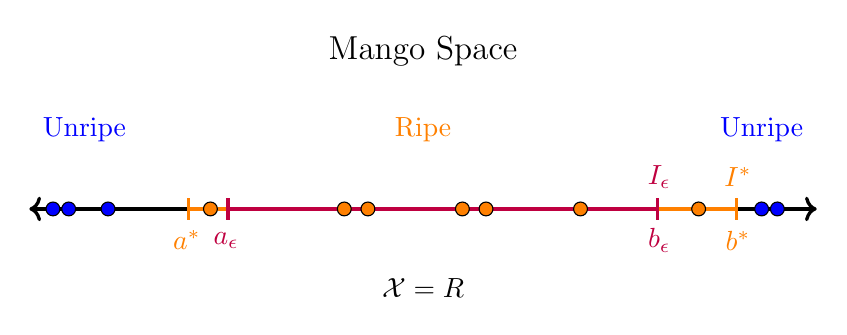
\begin{tikzpicture}
		\draw[<->,very thick] (-5,0) -- (5,0);
		\draw[color = orange, |-|,very thick] (-3,0) -- (4,0);
		\node[color=orange] at (4,.4) {$I^*$};
		\node at (0,2) {\large Mango Space} ;
		\node at (0,-1) {$\mathcal{X} = \mathbb{R}$} ;
		\node [color=blue] at (-4.3,1) {Unripe} ;
		\node [color=blue] at (4.3,1) {Unripe} ;
		\node [color=orange] at (0,1) {Ripe} ;

		\node [color=orange] at (-3,-.4) {$a^*$} ;
		\node [color=orange] at (4,-.4) {$b^*$} ;

		\draw [color=purple, |-|,very thick] (-2.5,0) -- (3,0);
		\node [color=purple] at (3,.4) {$I_\epsilon$} ;
		\node [color=purple] at (-2.5,-.4) {$a_\epsilon$} ;
		\node [color=purple] at (3,-.4) {$b_\epsilon$} ;

%		\draw [color=olive, |-|,very thick] (-3.5,0) -- (2.5,0);
%		\node [color=olive] at (3,.4) {$h_{\mathcal{T}}$} ;



		\node[circle,draw=black, fill=orange, inner sep=0pt,minimum size=5pt] at (2,0) {};
		\node[circle,draw=black, fill=orange, inner sep=0pt,minimum size=5pt] at (-1,0) {};
		\node[circle,draw=black, fill=orange, inner sep=0pt,minimum size=5pt] at (-.7,0) {};
		\node[circle,draw=black, fill=orange, inner sep=0pt,minimum size=5pt] at (.5,0) {};
		\node[circle,draw=black, fill=orange, inner sep=0pt,minimum size=5pt] at (.8,0) {};
		\node[circle,draw=black, fill=orange, inner sep=0pt,minimum size=5pt] at (-2.7,0) {};
		\node[circle,draw=black, fill=orange, inner sep=0pt,minimum size=5pt] at (3.5,0) {};

		\node[circle,draw=black, fill=blue, inner sep=0pt,minimum size=5pt] at (-4.5,0) {};
		\node[circle,draw=black, fill=blue, inner sep=0pt,minimum size=5pt] at (-4,0) {};
		\node[circle,draw=black, fill=blue, inner sep=0pt,minimum size=5pt] at (-4.7,0) {};
		\node[circle,draw=black, fill=blue, inner sep=0pt,minimum size=5pt] at (4.3,0) {};
		\node[circle,draw=black, fill=blue, inner sep=0pt,minimum size=5pt] at (4.5,0) {};
	\end{tikzpicture}
  \end{minipage}
  \vfill
  \begin{minipage}[t][0.5\textheight][t]{\textwidth}
Lets understand this visually.
$$
Err(x_0) = \sigma_\epsilon^2 + [E_\cT[\hat f(x_0)] - f(x_0)]^2 + E_\cT\big[ \hat{f}(x_0) - E_\cT[\hat{f}(x_0)] \big]^2\,.
$$\pause
Consider a data set, 
\end{minipage}
\end{frame}


\begin{frame}[fragile]{Point Variance of Linear Predictor}
Since $x_0^T  (\bfX^T\bfX)^{-1}\bfX^T\epsilon$ is a vector, squaring it is the same as multiply by its transpose. \pause This allow us to write
\begin{align*}
\action<+->{\textbf{Var} &= E_\cT\big[(\,x_0^T  (\bfX^T\bfX)^{-1}\bfX^T\epsilon\,)^2\big] && \text{From before,}}
\\
\action<+->{  &=   E_\cT\big[(\,x_0^T  (\bfX^T\bfX)^{-1}\bfX^T\epsilon\,)(\,x_0^T  (\bfX^T\bfX)^{-1}\bfX^T\epsilon\,)^T\big]  && }
\\
\action<+->{  &=   E_\cT\big[(\,x_0^T  (\bfX^T\bfX)^{-1}\bfX^T\epsilon\,)(\epsilon^T \bfX (\bfX^T\bfX)^{-1} \,x_0)\big] &&  }
\\
\action<+->{  &= (\,x_0^T  (\bfX^T\bfX)^{-1}\bfX^T) E_\cT[\epsilon\epsilon^T] (\bfX (\bfX^T\bfX)^{-1} x_0)  &&\bfX,\,x_0\,\text{const,}}
\\
\action<+->{  &=  (\,x_0^T  (\bfX^T\bfX)^{-1}\bfX^T)\,(\sigma_\epsilon^2 I)\, (\bfX (\bfX^T\bfX)^{-1} x_0)  && \text{Def. of Var,} }
\\
\action<+->{  &=  \sigma^2_\epsilon \, \,x_0^T  (\bfX^T\bfX)^{-1}x_0  && \text{Simplify.} }
\end{align*}
\action<+->{The variance is proportional to the variance in the random variable. But how do we understand the matrix $(\bfX^T\bfX)^{-1}$?}
\end{frame}







\begin{frame}[fragile]{Binary Classification}
  \begin{minipage}[t][0.5\textheight][t]{\textwidth}
	\centering \includegraphics[height=0.5\textheight]{L9BC2.png} 
  \end{minipage}
  \vfill
\begin{minipage}[t][0.5\textheight][t]{\textwidth}
In binary classification, the target space $\mathcal{Y}$ is a categorical variable with two labels. \pause For example, the data above (UW Breast Cancer Dataset) is attempting to classify tumor cells as malignant or nonmalignant based on the cells average area and average concavity. 

\end{minipage}
\end{frame}



















